\documentclass[conference]{IEEEtran}
\IEEEoverridecommandlockouts
% The preceding line is only needed to identify funding in the first footnote. If that is unneeded, please comment it out.
\usepackage{cite}
\usepackage{amsmath,amssymb,amsfonts}
\usepackage{algorithm}
\usepackage{algpseudocode}
\usepackage{graphicx}
\usepackage{listings}
\usepackage{sourcecodepro}
\usepackage{textcomp}
\usepackage{xcolor}

\lstset{
  basicstyle=\footnotesize\ttfamily,
  numbers=left,
  numberstyle=\tiny,
  frame=single,
  tabsize=2,
}

\begin{document}

\title{A Scalable Architecture for Massively Parallel Deep Learning}

\author{\IEEEauthorblockN{Jeff Hajewski}
\IEEEauthorblockA{\textit{Department of Computer Science} \\
\textit{University of Iowa}\\
Iowa City, IA, USA\\
jeffrey-hajewski@uiowa.edu}
\and
\IEEEauthorblockN{Suely Oliveira}
\IEEEauthorblockA{\textit{Department of Computer Science} \\
\textit{University of Iowa}\\
Iowa City, IA, USA \\
suely-oliveira@uiowa.edu}
}

\maketitle

\begin{abstract}

\end{abstract}

\begin{IEEEkeywords}
distributed deep learning, neural architecture search, artificial intelligence
\end{IEEEkeywords}

\section{Introduction}
Building robust and scalable distributed applications is challenging --- getting
communications patterns correct, handling node failures, and allowing for elastic
compute resources all contribute to a high level of complexity. These challenges
are exacerbated for long-runnining applications such as training large deep learning
models or neural architecture search. Among the many popular frameworks for
distributed programming, MPI \cite{Forum:1994:MMI:898758} combined with
additional accelerator paradigms such as OpenMP \cite{Dagum:1998:OIA:615255.615542},
OpenACC \cite{Wienke:2012:OFE:2402420.2402522}, and CUDA \cite{Nickolls:2008:SPP:1365490.1365500}
is the common choice for performance-critical numerical workloads. In the deep
learning setting, MPI is less popular with many favoring mutli-threading in
combination with multiple GPUs, and more recently experimenting with Kubernetes
\cite{8094194, 8672301}. Although part of this is simplicity of communication patterns,
the fault tolerance required for long-running model training (which can last on the
order of months in the industrial setting) makes MPI a poor choice for the underlying
communication infrastructure.

In this work we propose an RPC-based system for
distributed deep learning. We experiment with the proposed architecture in the domain
of neural architecture search (NAS), an extremely computationally intensive problem that
trains thousands of deep neural networks in search of an optimal network architecture.
Or system consists of four separate pieces: a \emph{model} that directs the search
for a network architecture, a number of \emph{workers} that perform the computational
work of training the models, a number of \emph{brokers} that form the backbone of
the data pipeline from model to workers, and a \emph{nameserver} that simplifies the
process of adding new brokers, workers, or models to the system. Our system offers
elastic compute resources, allowing an arbitrary number of workers to join during
high computational loads as well as allowing workers to leave the system, decreasing
the overall available compute, without needing to restart or manual intervention.
The system is fault-tolerant to the loss of workers or brokers, and is highly scalable
due to the ability of the brokers to share work and compute resources. Perhaps most
importantly from a usability perspective, our system is language agnostic. In our
experiments, we use Python for our model and workers, which we use to build and train
or deep neural networks via PyTorch \cite{paszke2017automatic}, and use Go to build
the data pipeline of brokers. We use gRPC \cite{Wang:1993:GCC:155870.155881} to handle
the generation of RPC stubs, but could have just as easily used Apache Thrift
\cite{Slee2007}, which generates stubs in a larger range of languages such as Ocaml,
Haskell, and Rust.

\section{Neural Architecture Search}
The goal of neural architecture search (NAS) is to find an optimal neural network
architecture for a given problem. NAS is computationally intensive due to the
requirement of having to train a candidate network in order to evaluate its
effectiveness. Although recent novel approaches have dramatically reduced this
cost \cite{DBLP:journals/corr/abs-1708-05344, pmlr-v80-pham18a}, these techniques
fix certain elements of the design process, somewhat limiting the available
architectures. Despite the computationally intense nature of the NAS problem,
the task itself is trivially parallelizable across the network evaluations ---
two separate networks can be trained simultaneously before being evaluated against
eachother.

The two common approaches to NAS are reinforcement learning based approaches such
as \cite{45826, Kyriakides:2018:NAS:3200947.3208068, pmlr-v80-pham18a}, and
evolutionary approaches such as \cite{DBLP:journals/corr/abs-1711-00436,
  DBLP:journals/corr/MiikkulainenLMR17, DBLP:conf/icml/RealMSSSTLK17}. In our
experiments we focus on the evolutionary approach due to its simplicity both in
understanding and implementation.

\subsection{Evolutionary Algorithms for NAS}
We use a relatively simple approach to evolving neural network architectures.
The problem domain we focus on is computer vision, so we restrict ourselves
to convolutional layers for the hidden layers. The last two layers of the
network are dense layer and are fixed to assure the number of categories
is sensible for the given classification task. The challenge with evolving
a neural network is in maintaining a valid neural network (a neural network
with a path from the input layer to the output layer). We maintain this
invariant as follows. Each time a layer is added to the network, it is
randomly connected to another layer in the network; however, there is
no guarantee that these two connected layers are part of the path from
the input layer to the output layer. It is possible they form a disconnected
subgraph of the network graph. We also maintain a phantom last layer --
it is not an actual layer but represents the first fixed last layer in
the formed network. Maintaining this phantom layer separate from the modified
layers allows us to always append layers without having to rearrange the
last layer.

\begin{algorithm}
  \caption{High-level outline of evolutionary algorithm.}\label{alg:evo-simple}
  \begin{algorithmic}[1]
    \Procedure{MutateNetwork}{}
    \State $\texttt{layer} \gets
    \texttt{RandomChoice}(\texttt{available\_layers})$
    \State $\texttt{this.layers.append(layer)}$
    \State $\texttt{this.connections.addRandomConnection}$
    \While {\textbf{not} $\texttt{this.nn.isConnected()}$}
    \State \text{Pick random layer and connect to last layer}
    \EndWhile
    \State \textbf{return} \texttt{GenerateNetwork(this.layers)}
    \EndProcedure
  \end{algorithmic}
\end{algorithm}

\section{RPC-based Communication}
Remote Procedure Call (RPC) offers a method of invoking a function on a remote
computer with a given set of arguments. Most RPC frameworks involve a DSL used
to define the RPC service, that is, the API available to the caller, and some
type of data serialization format. For example, gRPC uses Protocol Buffers
\cite{Varda2008} as the serialization format for data sent across the network.
RPC offers a number of advantages for network communication. It is robust to
node failures or network partitions (the RPC invokation simply fails). The data
sent across the network is compactly represented, giving way to high bandwidth
and low latency communication. The point-to-point communication allows for
diverse communication patterns and paradigms. RPC forms the network communication
infrastructure at Google \cite{van2017production}, Facebook \cite{Slee2007},
as well as Hadoop
\cite{Shvachko:2010:HDF:1913798.1914427, Lu:2013:HDH:2570457.2571128}.

While the robustness to node failures and finer-grained point-to-point
communication capabilities of RPC are core to building resilient
distributed systems, the more powerful feature we capitalize on is
the ability to build a system that is agnostic to the type of data
flowing through its pipes. Figure~\ref{fig:data-agnostic} gives an example
of constructing a Protocol Buffer[CITE] message type that can be used to
transport arbitrary data types through the system. Protocol Buffers (and
similarly, Thrift messages) support arbitrary length byte arrays
\footnote{In practice
  these arrays are limited in size. The failure rate of the RPC system
  typically increases with the size of the messages.} This means the
user can send a serialized object stored in the \texttt{Task}'s
\texttt{task\_obj} field without having to modify the system.
A user can switch between running models and tasks using Java to running
models and tasks using Python without modifying the system. In fact,
the system can transport and run these tasks (in both Java and Python)
simultaneously. By encapsulating the tasks (and results) as serialized
objects stored as byte arrays the entire system can be data type
agnostic.

\begin{figure}
  \begin{lstlisting}
message Task {
  string id = 1;
  enum type = 2; // or string type
  bytes task_obj = 3;
}
  \end{lstlisting}
  \caption{Example of a data agnostic message type.}\label{fig:data-agnostic}
\end{figure}

There is a slight catch. If information within the serialized object
is needed to properly schedule or transport the task/result to its
destination, this information will need to be added to the message
definition. This requires recompiling the message types and regenerating
the gRPC (or Thrift) stubs. This is a minor inconveninece, as incorporating
this new information into the system requires modifying the system
infrastructure.

\subsection{RPC vs MPI}

\section{System Architecture}
As previously mentioned, our system consists of four different components.
Figure~\ref{fig:sys-arch} shows an overview of the system architecture.
A model
is a problem specific implementation that controls what is sent to the system for
evaluation and handles the result it receives. The brokers form the data pipeline
of the system, moving work to available workers. Workers form the other customizable
part of the system because they need to know how to perform their assigned work.
Lastly, the nameserver maps known brokers to their network address -- this is useful
for connecting to brokers, such as a model connecting to a broker, a broker connecting
to a broker (for broker-broker peering), or a worker connecting to a broker. The
following sections will detail each components functionality individual and within
the system as a whole.

\begin{figure*}
  \centering
  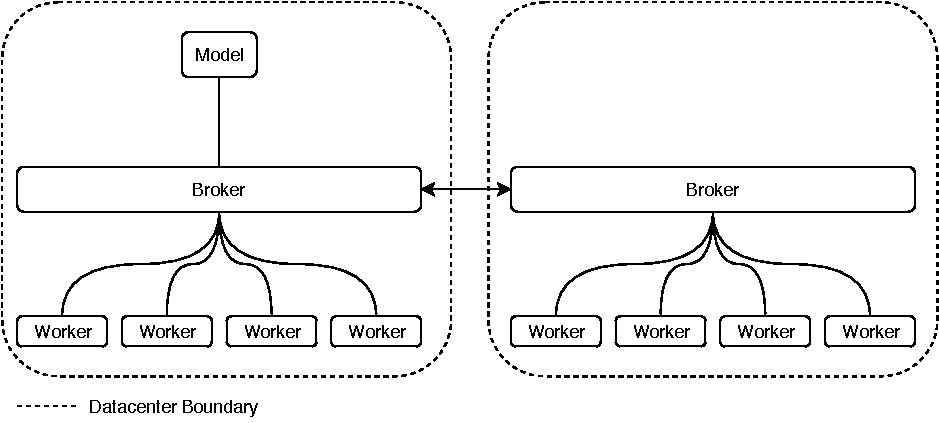
\includegraphics{img/broker-arch.pdf}
  \caption{Diagram of system architecture.}
  \label{fig:sys-arch}
\end{figure*}

\subsection{Model}
The model is the problem-specific, user-defined logic that determines what work
should be performed next and how the results of previously assigned work should
be processed. The only requirement of the model is that is uses a broker client
stub (generated by gRPC) to push work to the system and implements the model
service interface to allow the broker to push results back to the model.

The model needs to track outstanding tasks that have been sent to the broker.
While the system is fault-tolerant for most brokers and all workers, if the
broker the model is sending work to fails, the work the model is waiting to
receive will be lost and the model will need to resend to a new broker.

\subsection{Worker}
Workers are the other user-defined and implemented portion of the system. While
a single worker implementation can work for multiple model implementations, there
is no general worker implementation that will work across all languages and models.

\begin{figure}
  \begin{lstlisting}[language=python]
class BaseTask:
  def run(self):
    raise NotImplementedError()

class Worker:
  def process_task(self, task):
    result = task.run()
    self.broker_client.send_result(result)
  \end{lstlisting}
  \caption{Example Task API in Python.}\label{fig:python-api}
\end{figure}

Using an API similar to that shown in Figure~\ref{fig:python-api}, one can use
the same worker implementation for any task that inherits from the \texttt{BaseTask}
class.

\subsection{Nameserver}
The nameserver simplifies bookkeeping when starting new broker instances.
Rather than forcing the user to specify which brokers a newly started broker
should link up with, the nameserver stores and shares that information with
all registered brokers. During start-up, each broker registers with the nameserver
and begins sending heartbeat messages. The nameserver tracks which brokers have
sent heartbeats recently (via a user-modifiable timeout setting) and drops brokers
that have timed-out. If a broker sends a heartbeat \emph{after} the nameserver has
dropped the connection, the nameserver responds by telling the broker it must
re-register with the nameserver.

Brokers can request the nameserver send them an address of another broker with
which they can link and share resources. Rather than force the user to specify
which brokers should form a peering link, a broker will receive a random broker
address.

Care must be taken with the nameserver as this is the single point of failure
within the system. Although the system can continue to function without a
nameserver, new brokers will be unable to join. This means eventually the system
will fail as brokers leave the system (e.g., power outage, hardware failure, etc.).
The simple solution is to use an orchestration system such as Kubernetes to make
sure there is always at least one nameserver running. Because the nameserver
can force brokers to re-register, restoring a failed nameserver simply forces all
incoming heartbeat requests to re-register and thus restoring the state of the
nameserver broker registry prior to the crash. This mechanism greatly simplifies
the implementation of the nameserver. The only state that must persist between
crashes of the nameserver is that of the next available broker ID. If the nameserver
does not persist this to some type of durable medium (e.g., HDFS
\cite{Shvachko:2010:HDF:1913798.1914427}) then it is possible for multiple brokers
to receive the same broker ID.


\subsection{Broker}
Brokers form the data pipeline of our system. Work is sent from a model to a broker,
which in turn sends the work to a free worker and returns the result to the original
model. At its core, a broker is essentially just a process with a owned task queue,
a helper task queue (tasks received from other brokers), a processing queue, and
a results queue. Work in the owned task queue is work that was sent from a model directly
to the broker -- this is the work that will be lost if the broker crashes. Work in
the helper task queue is work that has been sent from other brokers that the respective
broker has agreed to help with. If the broker crashes, this work will \emph{not} be
lost as the other brokers will see the failure and can recover the task from their
processing queue. The processing queue stores tasks that have been sent to
workers or other brokers. When a result is received from a worker or another broker,
the corresponding ID will be removed from the processing queue and the result will
be added to the result queue. The broker pulls tasks from the result queue and sends
the result to its owner, which may be a model or another broker.

Brokers can establish links with other brokers.

\begin{figure}
  \centering
  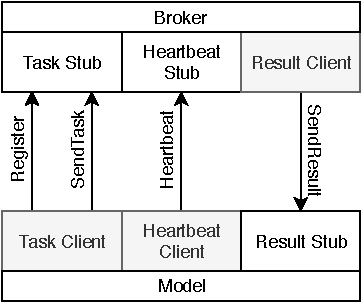
\includegraphics{img/model_broker}
  \caption{Communication pattern between the broker and
    model.}\label{fig:broker-model}
\end{figure}

\section{Experiments}

\section{Related Work}

\section{Conclusion}

\bibliographystyle{abbrv}
\bibliography{/home/jhaj/research/bibliographies/bdl,
  /home/jhaj/research/bibliographies/comps_plan}

\end{document}
